% =============================================================================
%  밴디트 문제와 행동 가치 추정 — 『밑바닥부터 시작하는 딥러닝 4』 1장 정리
%
%  컴파일:  tectonic -X compile ch01_bandit.tex
%  (XeLaTeX 계열 엔진 + kotex + NanumGothic 필요)
% =============================================================================
\documentclass[11pt,a4paper]{article}

\usepackage{kotex}
\usepackage{amsmath,amssymb}
\usepackage{graphicx}
\usepackage{booktabs}
\usepackage{multirow}
\usepackage{listings}
\usepackage{xcolor}
\usepackage{algorithm}
\usepackage{algpseudocode}
\usepackage[margin=27mm,top=28mm,bottom=28mm]{geometry}
\usepackage[labelsep=period,font=small,labelfont=bf]{caption}
\usepackage{enumitem}
\usepackage[hidelinks]{hyperref}

% ---- 한글 글꼴 -------------------------------------------------------------
\setmainhangulfont{NanumGothic}
\setsanshangulfont{NanumGothic}
\setmonohangulfont[Scale=MatchLowercase]{NanumGothic}

% ---- 한글 캡션 이름 ---------------------------------------------------------
\renewcommand{\figurename}{그림}
\renewcommand{\tablename}{표}
\renewcommand{\refname}{참고문헌}
\renewcommand{\abstractname}{초록}
\renewcommand{\contentsname}{차례}
\floatname{algorithm}{알고리즘}
\renewcommand{\algorithmicrequire}{\textbf{입력:}}
\renewcommand{\algorithmicensure}{\textbf{출력:}}

% ---- 코드 리스팅 -----------------------------------------------------------
\definecolor{codekw}{RGB}{0,86,153}
\definecolor{codecm}{RGB}{112,128,144}
\definecolor{codestr}{RGB}{163,21,21}
\definecolor{codebg}{RGB}{249,249,250}
% 주의: listings는 라틴 문자를 단어 단위로 버퍼링했다가 출력하는데, kotex 환경에서
% 한글이 섞이면 버퍼가 한글 뒤에 flush되어 글자 순서가 뒤바뀐다("q에" -> "에q").
% 그래서 한글 주석은 escapeinside 구간에서 일반 조판 모드로 넘겨 처리한다.
\lstdefinestyle{py}{
  language=Python,
  escapeinside={<@}{@>},
  basicstyle=\ttfamily\small,
  keywordstyle=\color{codekw}\bfseries,
  commentstyle=\color{codecm}\itshape,
  stringstyle=\color{codestr},
  backgroundcolor=\color{codebg},
  frame=single,
  rulecolor=\color{black!25},
  framesep=5pt,
  columns=fullflexible,
  keepspaces=true,
  showstringspaces=false,
  breaklines=true,
  captionpos=b,
  numbers=none,
  aboveskip=1.1em,
  belowskip=0.6em,
}
\lstset{style=py}
\renewcommand{\lstlistingname}{코드}

% ---- 그림 경로 -------------------------------------------------------------
\graphicspath{{../../images/figures/}{../../images/equations/}{../images/}}

% ---- 편의 매크로 -----------------------------------------------------------
\newcommand{\qt}{q}                       % 참값
\newcommand{\Qe}{Q}                       % 추정치
\newcommand{\E}{\mathbb{E}}
\newcommand{\eps}{\varepsilon}
\newcommand{\bookfig}[1]{\textit{출처: 원서 그림 #1.}}
\newcommand{\cmt}[1]{\textcolor{codecm}{#1}}   % 리스팅 안의 한글 주석

\title{\bfseries 밴디트 문제와 행동 가치 추정\\[2mm]
\large 탐색과 활용의 절충, 그리고 비정상 환경에서의 갱신 규칙}
\author{sajacaros\\\small \texttt{research@dacon.kr}}
\date{2026년 8월 16일}

\begin{document}
\maketitle

\begin{abstract}
\noindent
밴디트 문제는 에이전트의 행동이 환경의 상태를 바꾸지 않는, 강화 학습의 가장 단순한 형태다.
상태가 개입하지 않으므로 ``어떤 행동이 좋은가''라는 질문만 남고, 그 결과 강화 학습의 핵심 긴장인
\emph{탐색과 활용의 절충}을 다른 요소의 간섭 없이 관찰할 수 있다.
본고는 이 문제를 행동 가치 $\qt(A)=\E[R\mid A]$의 추정 문제로 정식화하고, 표본 평균에 기반한
추정치 $\Qe(A)$의 증분 갱신식을 유도한 뒤, $\eps$-탐욕 정책을 구현하여 실험한다.
이어 보상의 확률분포가 시간에 따라 변하는 \emph{비정상 문제}로 확장하여, 갱신 폭 $1/n$을 고정값
$\alpha$로 대체하는 것이 왜 지수 이동 평균에 해당하며 어떤 조건에서 이득인지를 보인다.
원서의 내용을 정리하는 데 그치지 않고 두 가지 보충 실험을 추가하였다.
첫째, $\eps$를 $0$부터 $1$까지 바꾸어 20,000걸음까지 관찰한 결과, 좋은 $\eps$는 문제의 성질이 아니라
\emph{플레이 길이}의 함수임을 확인하였다($\eps=0.01$이 약 7,500걸음에서 $\eps=0.1$을 추월한다).
둘째, 환경의 변화 속도 $\sigma$와 $\alpha$를 격자로 훑어, 고정값 $\alpha$의 우위가 $\alpha$의 크기 자체가
아니라 $\sigma>0$이라는 조건에서 비롯됨을 보였다. 나아가 참값 $\qt$를 그대로 아는 에이전트를 같은
잣대로 측정하여 \emph{성능 상한}을 구하고, $\sigma>0$에서 상위 $\alpha$들이 이미 상한에서 $0.001$ 이내에
도달해 있음을 확인하였다. 이는 승률이 $\alpha$를 선택하는 잣대로 부적절하며 $|\Qe-\qt|$와 같은 추정
오차가 필요함을 정량적으로 뒷받침한다.

\vspace{2mm}
\noindent\textbf{주제어:} 강화 학습, 멀티암드 밴디트, 행동 가치, $\eps$-탐욕 정책, 지수 이동 평균, 비정상 문제
\end{abstract}

\tableofcontents
\vspace{4mm}

% =============================================================================
\section{서론}
% =============================================================================

\subsection{머신러닝의 세 부류}

머신러닝은 학습에 쓰이는 신호의 성격에 따라 크게 셋으로 나뉜다.
\emph{지도 학습}(supervised learning)은 입력과 출력을 쌍으로 묶은 데이터로 학습하며, 각 입력에 대한
정답 레이블이 주어진다. \emph{비지도 학습}(unsupervised learning)에는 정답 레이블이 없고, 데이터에
숨어 있는 구조나 패턴을 찾는 것이 목적이다. 군집화, 특성 추출, 차원 축소가 여기에 속한다.

\begin{figure}[htbp]
\centering
\begin{minipage}[t]{0.48\linewidth}\centering
  \includegraphics[width=\linewidth]{{fig 1-1}.png}
\end{minipage}\hfill
\begin{minipage}[t]{0.48\linewidth}\centering
  \includegraphics[width=\linewidth]{{fig 1-2}.png}
\end{minipage}
\caption{지도 학습(왼쪽)과 비지도 학습(오른쪽). 전자는 입력--출력 쌍으로 학습하고, 후자는 레이블
없이 데이터의 구조를 찾는다. \bookfig{1-1, 1-2}}
\label{fig:sup-unsup}
\end{figure}

세 번째가 \emph{강화 학습}(reinforcement learning)이다. 여기에는 정답 레이블이 없는 대신 \emph{보상}이라는
신호가 있다. 에이전트가 환경에서 행동하면 환경은 보상과 상태를 돌려주고, 에이전트는 보상의 총합을
최대화하는 행동 방식, 즉 \emph{정책}을 스스로 찾는다. 그림~\ref{fig:rl-loop}이 이 상호작용을 보여준다.
주목할 점은 환경이 돌려주는 것이 \emph{보상}과 \emph{상태} 둘이라는 사실이다. 이 중 상태가 사라지면
문제는 결정적으로 단순해지는데, 그것이 바로 본고가 다루는 밴디트 문제다.

\begin{figure}[htbp]
\centering
\includegraphics[width=0.62\linewidth]{{fig 1-4}.png}
\caption{강화 학습에서 에이전트와 환경의 상호작용. 행동을 보내면 보상과 상태가 돌아온다.
\bookfig{1-4}}
\label{fig:rl-loop}
\end{figure}

\subsection{본고의 구성과 기여}

2절에서 밴디트 문제를 정식화하고 참값과 추정치의 표기를 정리한다. 3절에서 표본 평균에 기반한
가치 추정과 그 증분 구현을 유도하고, 4절에서 탐색과 활용의 절충 및 $\eps$-탐욕 정책을 다룬다.
5절은 구현, 6절은 정상 문제에서의 실험이다. 7절에서 비정상 문제로 확장한다.

원서\cite{dlfs4}의 정리에 더해 본고가 추가한 것은 다음 세 가지다.

\begin{enumerate}[leftmargin=*,itemsep=2pt]
  \item \textbf{$\eps$의 장기 거동}(\S\ref{sec:eps-exp}). 원서는 $\eps\in\{0.1,0.3,0.01\}$을 1,000걸음까지만
        비교한다. 본고는 $\eps=0$과 $\eps=1$이라는 두 극단을 포함해 20,000걸음까지 관찰하여, $\eps$의
        우열이 걸음 수에 따라 뒤집히는 지점을 특정한다.
  \item \textbf{$\alpha$와 $\sigma$의 격자 탐색}(\S\ref{sec:alpha-exp}). 원서는 $\sigma=0.1$인 환경에서
        $\alpha=0.8$ 하나만을 표본 평균과 견준다. 본고는 $\sigma$를 $0$부터 $0.1$까지 바꾸어, 고정값
        $\alpha$의 우위가 $\sigma>0$이라는 조건에 달려 있음을 보인다.
  \item \textbf{성능 상한의 측정}(\S\ref{sec:ceiling}). 참값 $\qt$를 그대로 아는 에이전트를 같은 잣대로
        측정하여, 승률이라는 잣대 자체가 어디서 천장에 막히는지를 수치로 제시한다.
\end{enumerate}

% =============================================================================
\section{문제 설정}
% =============================================================================

\subsection{밴디트 문제}

여러 대의 슬롯머신 중 어느 것을 플레이할지 고르는 문제를 \emph{밴디트 문제}라 한다. 슬롯머신을 뜻하는
속어 \texttt{one-armed bandit}(외팔이 강도)에서 온 이름이며, 여러 대를 동시에 다루므로
\emph{멀티암드 밴디트}(multi-armed bandit) 문제라고도 부른다. 슬롯머신마다 코인이 나올 확률이 다르지만
플레이어는 그 값을 모른다. 정해진 횟수 안에 얻는 보상의 총합을 최대로 만드는 것이 목표다.

\begin{figure}[htbp]
\centering
\includegraphics[width=0.62\linewidth]{{fig 1-6}.png}
\caption{밴디트 문제의 메커니즘. 그림~\ref{fig:rl-loop}과 달리 \emph{상태 화살표가 없고} 행동과 보상만
오간다. \bookfig{1-6}}
\label{fig:bandit-loop}
\end{figure}

이 문제가 강화 학습 중 가장 단순한 형태인 이유는 에이전트가 행동해도 환경의 상태가 변하지 않기
때문이다. 상태는 늘 같으므로 사실상 존재하지 않는 것과 같고, 에이전트는 상태를 고려하지 않은 채
``어떤 행동이 좋은가''만 생각하면 된다. 그림~\ref{fig:bandit-loop}에 상태 화살표가 없는 것이 그 시각적
표현이다. 문제의 구성 요소를 강화 학습의 용어로 옮기면 다음과 같다.

\begin{table}[htbp]
\centering
\caption{밴디트 문제의 구성 요소}
\label{tab:elements}
\small
\begin{tabular}{@{}ll@{}}
\toprule
강화 학습의 요소 & 밴디트 문제에서의 대응 \\
\midrule
환경(environment)   & 슬롯머신 \\
에이전트(agent)     & 플레이어 \\
행동(action)        & 어느 슬롯머신을 플레이할지 고르는 것 \\
보상(reward)        & 받은 코인 \\
상태(state)         & \textbf{없음}(항상 같은 상태로 취급) \\
\bottomrule
\end{tabular}
\end{table}

표~\ref{tab:elements}에서 상태를 ``없음''으로 둔 점은 강조할 만하다. 각 슬롯머신의 승률을 상태로
오해하기 쉬우나, 그것은 환경이 내부에 감춰둔 값일 뿐 에이전트가 받아 보는 신호가 아니다.
7절에서 그 승률이 시간에 따라 변하는 비정상 문제를 다루는데, 그때에도 에이전트에게 오는 것은
여전히 보상뿐이며 상태는 끝까지 등장하지 않는다.

\subsection{좋은 슬롯머신이란 무엇인가}

슬롯머신마다 얻을 수 있는 코인 개수의 확률분포가 정해져 있다. 그림~\ref{fig:dist}의 두 슬롯머신을
보자.

\begin{figure}[htbp]
\centering
\includegraphics[width=0.86\linewidth]{{fig 1-7}.png}
\caption{두 슬롯머신의 확률분포표. \bookfig{1-7}}
\label{fig:dist}
\end{figure}

좋은 슬롯머신이란 보상의 \emph{기댓값}(expected value)이 큰 슬롯머신이다. 그림~\ref{fig:dist}의 값으로
계산하면
\begin{align}
  \E[R\mid A=a] &= 0\times0.70 + 1\times0.15 + 5\times0.12 + 10\times0.03 = 1.05, \\
  \E[R\mid A=b] &= 0\times0.50 + 1\times0.40 + 5\times0.09 + 10\times0.01 = 0.95
\end{align}
이므로 $a$가 $b$보다 좋다.

문제는 플레이어가 이 확률분포를 모른다는 데 있다. 알 수 있는 것은 실제로 플레이해서 받은 보상뿐이며,
따라서 기댓값을 표본으로 추정해야 한다. 그런데 표본이 적으면 추정은 쉽게 뒤집힌다.
한 번씩만 플레이해 $a$에서 $0$, $b$에서 $1$을 받았다면 $b$가 좋아 보인다(그림~\ref{fig:samples} 왼쪽).
세 번씩 플레이하면 $a$의 표본 평균은 $(0+1+5)/3=2.0$, $b$는 $(1+0+0)/3=0.33$이 되어 순위가 뒤집힌다
(그림~\ref{fig:samples} 오른쪽). 플레이 횟수를 늘릴수록 표본 평균은 기댓값에 가까워진다.

\begin{figure}[htbp]
\centering
\begin{minipage}[t]{0.40\linewidth}\centering
  \includegraphics[width=\linewidth]{{fig 1-8}.png}
\end{minipage}\hfill
\begin{minipage}[t]{0.56\linewidth}\centering
  \includegraphics[width=\linewidth]{{fig 1-9}.png}
\end{minipage}
\caption{한 번씩 플레이한 결과(왼쪽)와 세 번씩 플레이한 결과(오른쪽). 표본이 적으면 추정 순위가
쉽게 뒤집힌다. \bookfig{1-8, 1-9}}
\label{fig:samples}
\end{figure}

\subsection{행동 가치와 표기}
\label{sec:notation}

보상을 확률 변수 $R$, 행동을 $A$로 표기하자. 행동 $A$를 취했을 때 받는 보상의 기댓값을
\emph{행동 가치}(action value)라 하고 다음과 같이 쓴다.
\begin{equation}
  \qt(A) = \E[R \mid A].
  \label{eq:action-value}
\end{equation}
앞의 예에서는 $\qt(a)=1.05$, $\qt(b)=0.95$이다. 이 표기 아래에서 밴디트 문제는 \emph{가치가 가장 큰
행동을 찾는 문제}로 요약된다.

다만 에이전트는 $\qt(A)$를 모르므로 추정치 $\Qe(A)$를 만들어 써야 한다. 본고는 원서를 따라
소문자 $\qt$를 환경이 갖고 있는 참값에, 대문자 $\Qe$를 에이전트가 짐작한 추정치에 일관되게 사용한다.
학습이란 결국 $\Qe(A)$를 $\qt(A)$에 가깝게 만드는 일이다.

\begin{table}[htbp]
\centering
\caption{참값, 추정치, 관측 승률의 구분}
\label{tab:qQ}
\small
\begin{tabular}{@{}llll@{}}
\toprule
표기 & 무엇인가 & 어떻게 정해지나 & 누가 아는가 \\
\midrule
참값 $\qt(A)$   & 행동 가치의 실제 값(= 진짜 승률) & 환경이 처음부터 갖고 있는 값 & 환경만 \\
추정치 $\Qe(A)$ & 에이전트가 짐작한 값             & 받은 보상으로 계산           & 에이전트 \\
관측 승률       & 실제로 이긴 비율                 & 보상 총합 $\div$ 플레이 횟수 & 둘 다 \\
\bottomrule
\end{tabular}
\end{table}

5절 이후의 구현에서 보상은 $0$(꽝) 또는 $1$(당첨) 두 값만 갖는다. 이 경우
\begin{equation}
  \qt(A) = \E[R\mid A] = P(R=1\mid A)
\end{equation}
이므로 행동 가치의 참값이 곧 그 슬롯머신의 진짜 승률이 된다. 이하에서 두 표현을 섞어 쓰는 것은
이 때문이다.

% =============================================================================
\section{가치 추정과 증분 구현}
% =============================================================================

\subsection{표본 평균}

$n$번 플레이해 보상 $R_1,\dots,R_n$을 받았다면, 행동 가치의 추정치는 표본 평균으로 둔다.
\begin{equation}
  \Qe_n = \frac{R_1+R_2+\cdots+R_n}{n}.
  \label{eq:sample-mean}
\end{equation}
큰 수의 법칙에 의해 시도 횟수 $n$이 커질수록 $\Qe_n$은 참값 $\qt$에 수렴한다.

식~\eqref{eq:sample-mean}을 그대로 구현하면 보상을 모두 저장해 두고 매번 전체 합을 다시 계산하게
된다. 메모리와 계산량이 모두 플레이 횟수 $n$에 비례해 늘어나므로 비효율적이다.

\subsection{증분 구현}

식~\eqref{eq:sample-mean}은 이전 추정치만으로 갱신할 수 있는 형태로 바꿀 수 있다. $n-1$번까지의
보상 총합이 $(n-1)\Qe_{n-1}$이라는 사실
\begin{equation}
  R_1+R_2+\cdots+R_{n-1} = (n-1)\,\Qe_{n-1}
  \label{eq:partial-sum}
\end{equation}
을 식~\eqref{eq:sample-mean}에 대입하면 다음을 얻는다.
\begin{align}
  \Qe_n &= \frac{1}{n}\bigl(\underbrace{R_1+\cdots+R_{n-1}}_{(n-1)\Qe_{n-1}} + R_n\bigr) \label{eq:inc-1}\\
        &= \frac{1}{n}\bigl\{(n-1)\Qe_{n-1} + R_n\bigr\} \nonumber\\
        &= \Bigl(1-\frac{1}{n}\Bigr)\Qe_{n-1} + \frac{1}{n}R_n \label{eq:inc-2}\\
        &= \Qe_{n-1} + \frac{1}{n}\bigl(R_n - \Qe_{n-1}\bigr). \label{eq:incremental}
\end{align}
식~\eqref{eq:incremental}이 \emph{증분 구현}(incremental implementation)이다. 이전 추정치 $\Qe_{n-1}$과
새로 받은 보상 $R_n$만 있으면 갱신할 수 있으므로 보상을 저장할 필요가 없고, 한 번의 갱신에 드는
계산량도 $n$에 무관하게 일정하다.

식~\eqref{eq:incremental}의 기하학적 의미는 명확하다. 그림~\ref{fig:numberline}처럼 수직선 위에서
$\Qe_{n-1}$을 $R_n$ 쪽으로 그 거리의 $1/n$만큼 옮기는 연산이다. $n$이 커질수록 이동 폭이 짧아지므로
갱신은 점점 둔해진다. 이 성질이 7절에서 비정상 문제를 다룰 때 결정적인 약점이 된다.

\begin{figure}[htbp]
\centering
\begin{minipage}[t]{0.52\linewidth}\centering
  \includegraphics[width=\linewidth]{{fig 1-10}.png}
\end{minipage}\hfill
\begin{minipage}[t]{0.44\linewidth}\centering
  \includegraphics[width=\linewidth]{{fig 1-11}.png}
\end{minipage}
\caption{식~\eqref{eq:incremental}의 두 가지 읽기. 왼쪽은 수직선 위에서 $R_n$ 쪽으로 $1/n$만큼
이동하는 연산으로, 오른쪽은 코드 한 줄로 본 것이다. \bookfig{1-10, 1-11}}
\label{fig:numberline}
\end{figure}

코드로는 \lstinline|Q = Q + (reward - Q) / n| 한 줄이면 된다. 예제
\texttt{s01\_avg.py}는 식~\eqref{eq:sample-mean}을 그대로 옮긴 기본 구현과 식~\eqref{eq:incremental}의
증분 구현이 같은 값을 내놓음을 확인한다.

% =============================================================================
\section{정책: 탐색과 활용}
% =============================================================================

추정치 $\Qe$가 준비되면 다음 질문은 그것을 어떻게 쓸 것인가이다. 가장 단순한 답은 추정치가 가장
큰 행동을 고르는 \emph{탐욕 정책}(greedy policy)으로, 지금까지 얻은 정보를 최대한 써먹는다는 뜻에서
\emph{활용}(exploitation)이라 부른다. 그러나 추정치는 부정확할 수 있고, 특히 초반에 우연히 좋아 보인
슬롯머신에 갇히면 그 오해를 스스로 교정할 기회가 사라진다.

반대편에 \emph{탐색}(exploration)이 있다. 추정치와 무관하게 다른 슬롯머신도 시도해 정보를 모으는
것으로, 당장의 보상은 손해지만 추정치의 정확도가 올라간다. 활용과 탐색은 한쪽을 늘리면 다른 쪽이
줄어드는 \emph{상충 관계}(trade-off)에 있다.

가장 단순한 절충안이 \emph{$\eps$-탐욕 정책}($\eps$-greedy policy)이다. 확률 $\eps$로 무작위 행동을
취하고(탐색), 확률 $1-\eps$로 추정치가 최대인 행동을 취한다(활용). 예컨대 $\eps=0.1$이면 10번 중
1번은 무작위로 플레이한다.

\begin{algorithm}[htbp]
\caption{$\eps$-탐욕 정책에 의한 밴디트 학습}
\label{alg:eps-greedy}
\begin{algorithmic}[1]
\Require 슬롯머신 대수 $K$, 탐색 확률 $\eps$, 총 걸음 수 $T$
\State $\Qe(a) \gets 0$, $n(a) \gets 0$ \quad ($a=1,\dots,K$)
\For{$t = 1$ \textbf{to} $T$}
  \State $u \sim \mathrm{Uniform}(0,1)$
  \If{$u < \eps$}
    \State $A_t \gets$ $\{1,\dots,K\}$에서 균등하게 뽑은 행동 \Comment{탐색}
  \Else
    \State $A_t \gets \arg\max_a \Qe(a)$ \Comment{활용}
  \EndIf
  \State 환경에서 보상 $R_t$를 받는다
  \State $n(A_t) \gets n(A_t) + 1$
  \State $\Qe(A_t) \gets \Qe(A_t) + \dfrac{1}{n(A_t)}\bigl(R_t - \Qe(A_t)\bigr)$
         \Comment{식~\eqref{eq:incremental}}
\EndFor
\end{algorithmic}
\end{algorithm}

% =============================================================================
\section{구현}
% =============================================================================

\subsection{환경: 슬롯머신}

환경은 \texttt{Bandit} 클래스가 맡는다. 생성 시 각 슬롯머신의 승률을 $[0,1)$의 무작위값으로
초기화하고, \texttt{play(arm)}은 \texttt{arm}번째 슬롯머신을 플레이해 그 승률의 확률로 $1$을,
아니면 $0$을 반환한다.

\begin{lstlisting}[caption={환경 구현 (\texttt{s02\_bandit.py})},label={lst:bandit}]
class Bandit:
    def __init__(self, arms=10):  <@\cmt{\# arms = 슬롯머신 대수}@>
        self.rates = np.random.rand(arms)  <@\cmt{\# 각 슬롯머신의 승률 = 참값 q}@>

    def play(self, arm):
        rate = self.rates[arm]
        if rate > np.random.rand():
            return 1
        else:
            return 0
\end{lstlisting}

여기서 \texttt{self.rates[arm]}이 \S\ref{sec:notation}에서 말한 참값 $\qt(A)$, 곧 그 슬롯머신의 진짜
승률이다. 이 배열에 대해 네 가지를 분명히 해 둘 필요가 있다.
첫째, \texttt{Bandit()}을 만드는 순간 값이 정해지고 그 판이 끝날 때까지 바뀌지 않는다(정상 문제).
둘째, 데이터로 계산한 값이 아니라 환경이 처음부터 갖고 있는 값이며, 에이전트는 이 배열을 볼 수 없다.
에이전트에게 주어지는 것은 오직 $0$ 또는 $1$의 보상뿐이고, 그것만으로 \texttt{rates}$(=\qt)$를 짐작한
\texttt{Qs}$(=\Qe)$를 만들어야 한다.
셋째, \texttt{Bandit()}을 새로 만들 때마다 승률이 다시 뽑히므로 실험마다 문제의 난이도가 달라진다.
넷째, 그럼에도 우리가 참값 $\qt$를 알고 있는 것은 이것이 시뮬레이션이기 때문이며, 덕분에
$|\Qe-\qt|$ 같은 추정 오차를 잴 수 있다. \S\ref{sec:ceiling}의 성능 상한 측정도 같은 특권에 기댄다.

\subsection{에이전트: 플레이어}

에이전트는 각 슬롯머신의 가치 추정치 \texttt{Qs}와 플레이 횟수 \texttt{ns}를 들고 다니며,
\texttt{update()}에서 식~\eqref{eq:incremental}로 추정치를 갱신하고 \texttt{get\_action()}에서
$\eps$-탐욕 정책으로 행동을 고른다.

\begin{lstlisting}[caption={에이전트 구현 (\texttt{s02\_bandit.py})},label={lst:agent}]
class Agent:
    def __init__(self, epsilon, action_size=10):
        self.epsilon = epsilon  <@\cmt{\# 무작위로 행동할 확률(탐색 확률)}@>
        self.Qs = np.zeros(action_size)  <@\cmt{\# 참값 q에 대한 추정치 Q}@>
        self.ns = np.zeros(action_size)

    <@\cmt{\# 슬롯머신의 가치 추정}@>
    def update(self, action, reward):
        self.ns[action] += 1
        self.Qs[action] += (reward - self.Qs[action]) / self.ns[action]

    <@\cmt{\# 행동 선택($\eps$-탐욕 정책)}@>
    def get_action(self):
        if np.random.rand() < self.epsilon:
            return np.random.randint(0, len(self.Qs))  <@\cmt{\# 무작위 행동 선택}@>
        return np.argmax(self.Qs)  <@\cmt{\# 탐욕 행동 선택}@>
\end{lstlisting}

% =============================================================================
\section{실험: 정상 문제}
% =============================================================================

\subsection{한 번의 실행}

슬롯머신 10대, $\eps=0.1$, 1,000걸음으로 알고리즘~\ref{alg:eps-greedy}을 한 번 실행한다. 한 걸음은
행동 선택 $\rightarrow$ 플레이하여 보상 획득 $\rightarrow$ 추정치 갱신의 세 단계로 이루어진다.

\begin{figure}[htbp]
\centering
\begin{minipage}[t]{0.49\linewidth}\centering
  \includegraphics[width=\linewidth]{{fig 1-12}.png}
\end{minipage}\hfill
\begin{minipage}[t]{0.49\linewidth}\centering
  \includegraphics[width=\linewidth]{{fig 1-13}.png}
\end{minipage}
\caption{단일 실행의 결과. 왼쪽은 보상 총합, 오른쪽은 그 기울기에 해당하는 평균 승률
(누적 보상 $\div$ 걸음 수)이다. \bookfig{1-12, 1-13}}
\label{fig:single-run}
\end{figure}

그림~\ref{fig:single-run} 왼쪽에서 보상 총합의 기울기가 곧 승률이다. 120걸음 부근에서 한 번 꺾인 뒤로는
거의 직선인데, 좋은 슬롯머신을 찾아 계속 당기고 있다는 뜻이다. 같은 정보를 승률로 그린 것이 오른쪽으로,
120걸음 부근까지는 표본이 적어 $0.2$에서 $0.4$ 사이를 크게 오르내리다가, 이후 꾸준히 올라 600걸음
무렵 $0.8$을 넘어서고 그 뒤로는 완만하게 안정된다.

단, 슬롯머신의 승률과 플레이 결과가 모두 무작위이므로 이 그림은 실행할 때마다 달라진다.

\subsection{알고리즘의 평균적 특성}

같은 알고리즘을 10번 돌린 결과를 겹쳐 그리면(그림~\ref{fig:ten-runs}) 1,000걸음 시점에서 승률이
$0.6$대부터 $0.95$까지 세로로 넓게 흩어진다. 알고리즘이 같은데도 이렇게 벌어지는 것은 슬롯머신의
승률이 실험마다 다르게 뽑히기 때문이다. 따라서 한 번의 결과로는 알고리즘의 성능을 판단할 수 없다.

\begin{figure}[htbp]
\centering
\begin{minipage}[t]{0.49\linewidth}\centering
  \includegraphics[width=\linewidth]{{fig 1-14}.png}
\end{minipage}\hfill
\begin{minipage}[t]{0.49\linewidth}\centering
  \includegraphics[width=\linewidth]{{fig 1-15}.png}
\end{minipage}
\caption{10번의 실행을 겹쳐 그린 결과(왼쪽)와 평균을 내는 방향(오른쪽). 평균은 한 실험의 시간축이
아니라 \emph{같은 걸음 수끼리} 세로로 낸다. \bookfig{1-14, 1-15}}
\label{fig:ten-runs}
\end{figure}

해법은 여러 번 실험하고 \emph{각 걸음마다} 평균을 내는 것이다. 그림~\ref{fig:ten-runs} 오른쪽의
빨간 화살표가 그 방향을 보여준다. 1걸음 시점은 1걸음 시점끼리, 1000걸음 시점은 1000걸음 시점끼리
묶는다. 구현에서는 200번의 실험 결과를 $(200, 1000)$ 형상의 배열 \texttt{all\_rates}에 쌓고
\texttt{np.average(all\_rates, axis=0)}으로 평균한다.

\begin{figure}[htbp]
\centering
\begin{minipage}[t]{0.49\linewidth}\centering
  \includegraphics[width=\linewidth]{{fig 1-16}.png}
\end{minipage}\hfill
\begin{minipage}[t]{0.49\linewidth}\centering
  \includegraphics[width=\linewidth]{{fig 1-17}.png}
\end{minipage}
\caption{200번 실험의 걸음별 평균 승률(왼쪽)과 $\eps$를 세 가지로 바꾼 비교(오른쪽).
\bookfig{1-16, 1-17}}
\label{fig:avg-runs}
\end{figure}

그 결과가 그림~\ref{fig:avg-runs} 왼쪽이다. 그림~\ref{fig:single-run}의 출렁임이 사라지고 매끄러운
곡선이 남는다. $y$축이 $0.5$에서 시작하는 것은 아무것도 모르는 상태에서 무작위로 고른 것과 같은
승률이기 때문이며, 이 곡선이 이 알고리즘의 ``평균적인 실력''이다.

$\eps$를 $0.1$, $0.3$, $0.01$로 바꾸어 비교하면(그림~\ref{fig:avg-runs} 오른쪽) 150걸음 부근에서
$\eps=0.1$이 $\eps=0.3$을 추월하는 교차점이 나타난다. 교차점 왼쪽에서는 탐색을 많이 하는 $\eps=0.3$이
좋은 슬롯머신을 빨리 찾아 앞서지만, 오른쪽에서는 다 찾은 뒤에도 30\%씩 딴 데를 당기는 비용이 쌓여
뒤처진다. $\eps=0.01$은 1,000걸음 내내 오르는 중이어서 아직 학습이 끝나지 않았음을 보여준다.
이 마지막 관찰이 다음 절의 출발점이다.

\subsection{[보충] $\eps$의 장기 거동}
\label{sec:eps-exp}

원서는 $\eps=0.01$이 ``아직 오르는 중''이라는 관찰에서 멈춘다. 그렇다면 충분히 오래 플레이하면
$\eps=0.01$이 $\eps=0.1$을 따라잡는가? 이를 확인하기 위해 두 실험을 수행하였다
\footnote{실험 스크립트: \texttt{s04\_epsilon\_comparison.py}.} 첫째, $\eps\in\{0, 0.01, 0.1, 0.3, 1\}$로 200회 실험 $\times$
1,000걸음. 둘째, $\eps\in\{0.01, 0.1\}$로 100회 실험 $\times$ 20,000걸음.

\begin{table}[htbp]
\centering
\caption{정상 문제에서 $\eps$에 따른 평균 승률. 왼쪽 두 열은 200회 실험 $\times$ 1,000걸음,
오른쪽 네 열은 100회 실험 $\times$ 20,000걸음의 결과다. 각 열의 최댓값을 굵게 표시하였다.}
\label{tab:eps}
\small
\begin{tabular}{@{}lcc@{\hskip 8mm}cccc@{}}
\toprule
& \multicolumn{2}{c}{1,000걸음 실험} & \multicolumn{4}{c}{20,000걸음 실험} \\
\cmidrule(r){2-3}\cmidrule(l){4-7}
$\eps$ & 100걸음 & 1,000걸음 & 1,000걸음 & 5,000걸음 & 10,000걸음 & 20,000걸음 \\
\midrule
$0$    & 0.4856 & 0.4862 & --- & --- & --- & --- \\
$0.01$ & 0.5630 & 0.7414 & 0.7177 & \textbf{0.8386} & \textbf{0.8667} & \textbf{0.8819} \\
$0.1$  & \textbf{0.7137} & \textbf{0.8441} & \textbf{0.8344} & 0.8545 & 0.8577 & 0.8596 \\
$0.3$  & 0.7111 & 0.7710 & --- & --- & --- & --- \\
$1$    & 0.4882 & 0.4918 & --- & --- & --- & --- \\
\bottomrule
\end{tabular}
\end{table}

\begin{figure}[htbp]
\centering
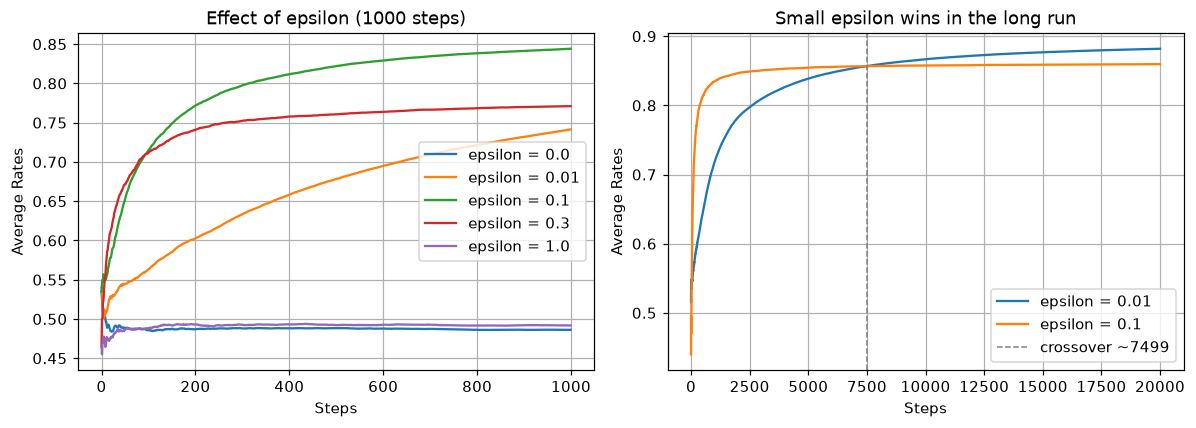
\includegraphics[width=\linewidth]{s04_epsilon_comparison.png}
\caption{$\eps$에 따른 평균 승률. 왼쪽은 1,000걸음까지, 오른쪽은 20,000걸음까지이며 회색 점선이
$\eps=0.01$과 $\eps=0.1$의 교차점이다. 난수 시드를 $0$으로 고정하여 재현 가능하다.}
\label{fig:eps-comp}
\end{figure}

표~\ref{tab:eps}과 그림~\ref{fig:eps-comp}에서 세 가지를 읽을 수 있다.

첫째, 두 극단은 모두 실패한다. $\eps=0$(활용만)과 $\eps=1$(탐색만)은 1,000걸음 뒤에도 각각
$0.4862$와 $0.4918$로, 무작위로 고른 것과 다를 바 없는 $0.5$ 근처에 머문다. 실패의 이유는 정반대다.
$\eps=0$은 처음 좋아 보인 슬롯머신에 갇혀 더 나은 것을 찾지 못하고, $\eps=1$은 찾아 놓고도 쓰지 않는다.
학습이 일어나려면 탐색과 활용이 함께 있어야 한다.

둘째, 1,000걸음까지는 $\eps=0.1$이 $0.8441$로 압도적이지만 그것이 최종 순위는 아니다. 20,000걸음
실험에서 $\eps=0.1$은 $0.8596$에서 사실상 포화하는 반면 $\eps=0.01$은 계속 올라 $0.8819$에 이른다.
역전이 확정되는 지점은 7,499걸음이다.

셋째, 이 역전은 비용과 이득의 시간 구조에서 나온다. 탐색에 드는 비용은 매 걸음 $\eps$의 확률로
일정하게 발생하지만, 탐색으로 찾아낸 이득은 남은 걸음 내내 쌓인다. 그러므로 오래 플레이할수록 작은
$\eps$가 유리해진다. 요컨대 ``좋은 $\eps$''는 문제의 성질이 아니라 \emph{얼마나 오래 플레이하는가}에
달려 있다.

% =============================================================================
\section{비정상 문제}
% =============================================================================

\subsection{표본 평균의 한계}

지금까지는 보상의 확률분포가 변하지 않는 \emph{정상 문제}(stationary problem)를 다루었다. 현실의
많은 문제는 시간이 지나면서 확률분포가 변하는 \emph{비정상 문제}(non-stationary problem)다. 이때는
오래된 보상일수록 현재의 가치를 제대로 반영하지 못하므로 최근 보상을 더 중시해야 한다.

그런데 표본 평균은 모든 보상을 똑같은 비중으로 다룬다. 그림~\ref{fig:weights} 왼쪽에서 막대 높이가
전부 같은 것이 그 표현으로, 1,000번째 보상과 첫 번째 보상의 발언권이 동일하다. 승률이 변하는
환경에서는 이미 낡은 $R_1$이 현재 추정치를 계속 붙잡고 있는 셈이다.

\begin{figure}[htbp]
\centering
\begin{minipage}[t]{0.47\linewidth}\centering
  \includegraphics[width=\linewidth]{{fig 1-18}.png}
\end{minipage}\hfill
\begin{minipage}[t]{0.49\linewidth}\centering
  \includegraphics[width=\linewidth]{{fig 1-19}.png}
\end{minipage}
\caption{각 보상에 붙는 가중치. 표본 평균(왼쪽)은 모든 보상을 동일하게 다루지만, 고정값 $\alpha$
(오른쪽)는 최근 보상에 비중을 몰아준다. \bookfig{1-18, 1-19}}
\label{fig:weights}
\end{figure}

\subsection{고정값 $\alpha$와 지수 이동 평균}

해법은 식~\eqref{eq:incremental}의 갱신 폭 $1/n$을 고정값 $\alpha\in(0,1]$로 바꾸는 것이다.
\begin{equation}
  \Qe_n = \Qe_{n-1} + \alpha\bigl(R_n - \Qe_{n-1}\bigr).
  \label{eq:alpha-update}
\end{equation}
이 식이 실제로 최근 보상에 더 큰 비중을 준다는 것은 전개해 보면 드러난다. 먼저
식~\eqref{eq:alpha-update}을 정리하면
\begin{equation}
  \Qe_n = \alpha R_n + (1-\alpha)\Qe_{n-1}
  \label{eq:alpha-1}
\end{equation}
이고, 같은 식을 한 단계 앞에 적용하면 $\Qe_{n-1} = \alpha R_{n-1} + (1-\alpha)\Qe_{n-2}$이다.
이를 식~\eqref{eq:alpha-1}에 대입하면
\begin{equation}
  \Qe_n = \alpha R_n + \alpha(1-\alpha)R_{n-1} + (1-\alpha)^2 \Qe_{n-2}
\end{equation}
이 되고, 이 대입을 끝까지 반복하면 다음을 얻는다.
\begin{equation}
  \Qe_n = \alpha R_n + \alpha(1-\alpha)R_{n-1} + \cdots
          + \alpha(1-\alpha)^{n-1}R_1 + (1-\alpha)^n \Qe_0.
  \label{eq:ema}
\end{equation}
즉 $k$걸음 전의 보상 $R_{n-k}$에는 $\alpha(1-\alpha)^k$의 가중치가 붙는다. $0<\alpha\le 1$이므로
가중치는 과거로 갈수록 \emph{지수적으로 감소}하며, 초깃값 $\Qe_0$의 영향도 $(1-\alpha)^n$으로 함께
사라진다. 이런 갱신 방식을 \emph{지수 이동 평균}(exponential moving average)이라 한다.
그림~\ref{fig:weights} 오른쪽이 식~\eqref{eq:ema}의 가중치를 그린 것으로, 왼쪽과 같은 축인데 막대가
오른쪽으로 갈수록 높아진다. 감소 속도를 정하는 손잡이가 $\alpha$이며, 이 손잡이를 어떻게 돌릴지가
\S\ref{sec:alpha-exp}의 주제다.

\subsection{구현}

비정상 환경은 \texttt{NonStatBandit}이 흉내 낸다. 플레이할 때마다 모든 슬롯머신의 승률에 표준편차
$\sigma$의 정규 노이즈를 더해 참값 $\qt$가 조금씩 흔들리게 한다. $\sigma$는 환경의 변화 속도이며,
$\sigma=0$이면 정상 문제와 같아진다. 승률에 별도의 절단을 두지 않으므로 $\sigma$가 크면 참값이
$1$을 넘거나 $0$ 아래로 내려갈 수 있다는 점은 결과를 읽을 때 유의해야 한다.

\begin{lstlisting}[caption={비정상 환경 (\texttt{s05\_\allowbreak non\_\allowbreak stationary.py})},label={lst:nonstat}]
class NonStatBandit:
    def __init__(self, arms=10, sigma=0.1):
        self.arms = arms
        self.sigma = sigma  <@\cmt{\# 참값 q가 한 걸음마다 흔들리는 정도}@>
        self.rates = np.random.rand(arms)  <@\cmt{\# 각 슬롯머신의 참값 q}@>

    def play(self, arm):
        rate = self.rates[arm]
        self.rates += self.sigma * np.random.randn(self.arms)  <@\cmt{\# 노이즈 추가}@>
        if rate > np.random.rand():
            return 1
        else:
            return 0
\end{lstlisting}

에이전트 쪽은 \texttt{update()}만 식~\eqref{eq:alpha-update}으로 바꾸면 된다. 플레이 횟수 \texttt{ns}가
더 이상 필요 없다는 점도 눈에 띈다. 행동 선택 \texttt{get\_action()}은 \texttt{Agent}와 동일한
$\eps$-탐욕 정책이다.

\begin{lstlisting}[caption={고정값 $\alpha$ 에이전트 (\texttt{s05\_\allowbreak non\_\allowbreak stationary.py})},label={lst:alpha}]
class AlphaAgent:
    def __init__(self, epsilon, alpha, actions=10):
        self.epsilon = epsilon
        self.Qs = np.zeros(actions)  <@\cmt{\# 참값 q에 대한 추정치 Q}@>
        self.alpha = alpha  <@\cmt{\# 고정값 $\alpha$}@>

    def update(self, action, reward):
        <@\cmt{\# $\alpha$로 갱신}@>
        self.Qs[action] += (reward - self.Qs[action]) * self.alpha
\end{lstlisting}

\subsection{표본 평균과 고정값 $\alpha$의 비교}

$\sigma=0.1$인 비정상 환경에서 표본 평균 방식과 $\alpha=0.8$ 방식을 200회 실험으로 비교한 결과가
그림~\ref{fig:nonstat}이다.

\begin{figure}[htbp]
\centering
\includegraphics[width=0.68\linewidth]{{fig 1-20}.png}
\caption{비정상 문제($\sigma=0.1$)에서 표본 평균과 $\alpha=0.8$의 비교. 200회 실험의 걸음별 평균이다.
\bookfig{1-20}}
\label{fig:nonstat}
\end{figure}

초반에는 두 곡선이 거의 겹친다. 표본 평균도 $n$이 작을 때는 갱신 폭 $1/n$이 커서 변화를 잘 따라가기
때문이다. 그러나 200걸음 부근부터 갈라지기 시작해 끝까지 간격이 벌어진다. $n$이 커지면서 $1/n$이 $0$에
가까워져 표본 평균은 사실상 학습을 멈추는 반면, 고정값 $\alpha$는 언제나 같은 보폭으로 최근 보상을
따라가기 때문이다.

다만 이 그림은 $\sigma=0.1$이라는 \emph{하나의} 환경에서 $\alpha=0.8$이라는 \emph{하나의} 값을 쓴
결과라는 점에 유의해야 한다. 이것만 보면 ``$\alpha$는 클수록 좋다''로 읽히기 쉽다. 다음 절이 그
해석을 검증한다.

\subsection{[보충] $\alpha$와 환경 변화 속도 $\sigma$}
\label{sec:alpha-exp}

$\alpha\in\{0.01,0.03,0.1,0.3,0.8\}$와 $\sigma\in\{0,0.01,0.03,0.1\}$의 격자에 대해, 각 조건에서 200회
실험 $\times$ 1,000걸음을 수행하고 뒤쪽 절반 구간(500\,--\,1,000걸음)의 평균 보상을 측정하였다
\footnote{실험 스크립트: \texttt{s06\_alpha\_comparison.py}.} 앞쪽 절반을 제외한 것은 초반이 느린 작은 $\alpha$가 학습 구간
때문에 부당하게 손해 보는 것을 막기 위해서다.

\begin{table}[htbp]
\centering
\caption{$\sigma$별 정상 구간(뒤쪽 절반) 평균 보상. 각 행에서 고정값 $\alpha$ 중 최고를 굵게,
표본 평균이 그 행 전체의 최고일 때 밑줄로 표시하였다. `상한'은 참값 $\qt$를 그대로 아는 에이전트를 같은 조건에서 측정한 값이다(\S\ref{sec:ceiling}).
행끼리의 비교는 의미가 없다.}
\label{tab:alpha-grid}
\small
\begin{tabular}{@{}lccccc@{\hskip 6mm}cc@{}}
\toprule
& \multicolumn{5}{c}{고정값 $\alpha$} & \multirow{2}{*}{표본 평균} & \multirow{2}{*}{상한} \\
\cmidrule(r){2-6}
$\sigma$ & $0.01$ & $0.03$ & $0.1$ & $0.3$ & $0.8$ & & \\
\midrule
$0$     & 0.6031 & 0.6712 & 0.8268 & \textbf{0.8305} & 0.8220 & \underline{0.8612} & 0.8627 \\
$0.01$  & 0.6306 & 0.7226 & 0.8475 & 0.8931 & \textbf{0.9052} & 0.8703 & 0.9092 \\
$0.03$  & 0.7445 & 0.8099 & 0.9148 & 0.9361 & \textbf{0.9444} & 0.9000 & 0.9449 \\
$0.1$   & 0.7784 & 0.8760 & 0.9347 & \textbf{0.9464} & 0.9445 & 0.9069 & 0.9474 \\
\bottomrule
\end{tabular}
\end{table}

\begin{figure}[htbp]
\centering
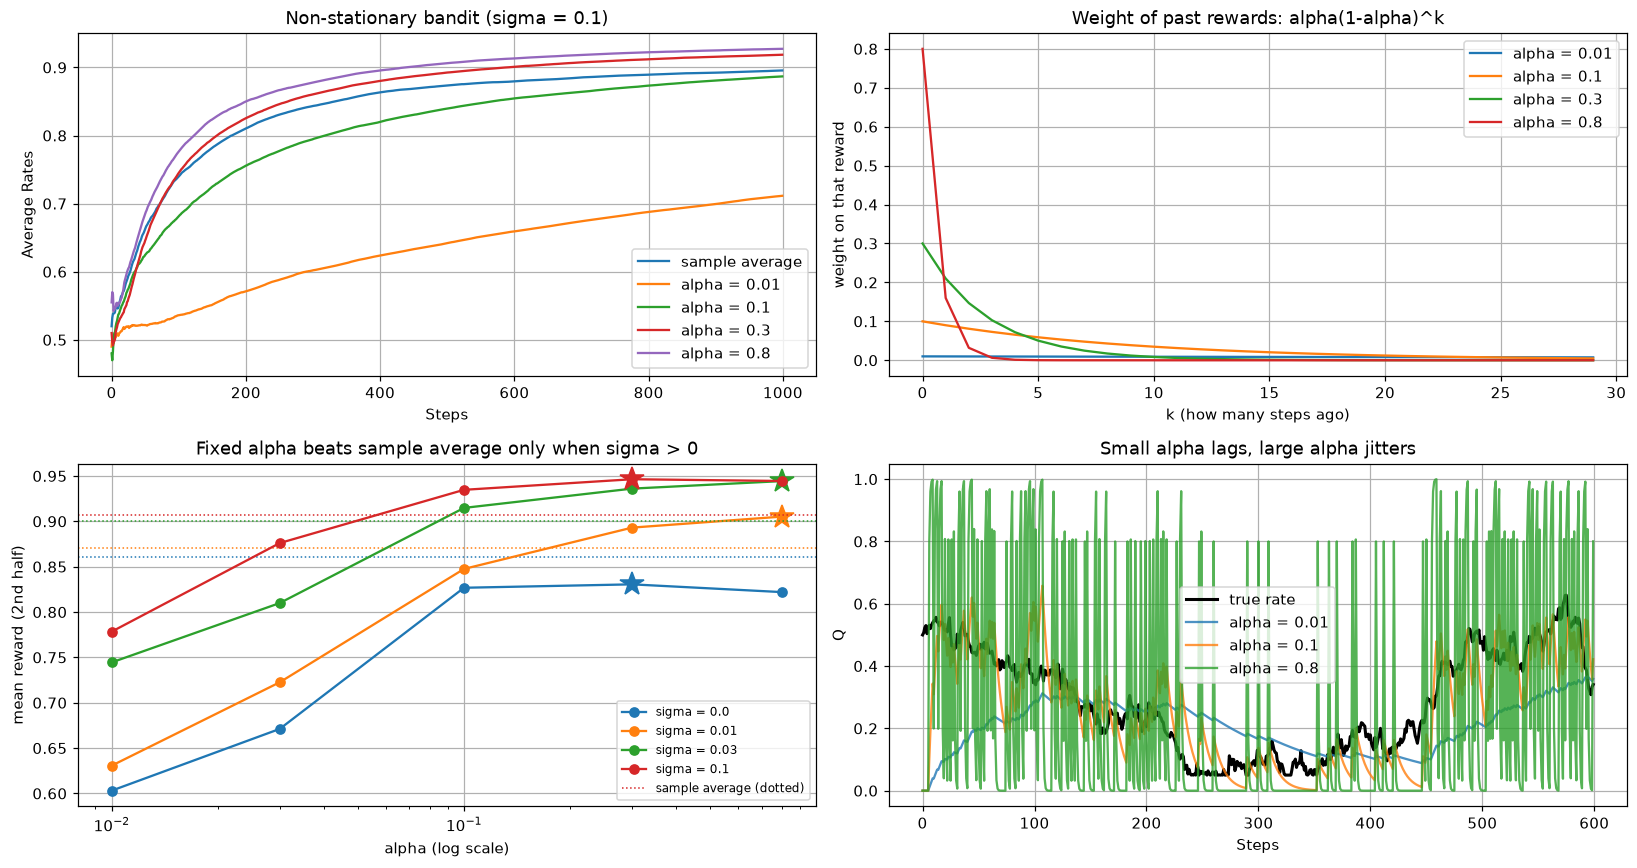
\includegraphics[width=\linewidth]{s06_alpha_comparison.png}
\caption{$\alpha$ 비교의 네 국면. 왼쪽 위는 $\sigma=0.1$에서의 승률 추이, 오른쪽 위는 과거 보상에
붙는 가중치 $\alpha(1-\alpha)^k$, 왼쪽 아래는 $\sigma$별 최적 $\alpha$(점선은 같은 색 $\sigma$에서
표본 평균이 낸 점수), 오른쪽 아래는 슬롯머신 한 대만 떼어내 추정치 $\Qe$가 참값 $\qt$를 쫓아가는
모습이다.}
\label{fig:alpha-comp}
\end{figure}

표~\ref{tab:alpha-grid}의 핵심은 각 행에서 굵게 표시한 값과 `표본 평균' 열의 대소 관계다.
$\sigma=0$인 첫 행에서만 표본 평균($0.8612$)이 모든 고정값 $\alpha$를 앞선다. 승률이 변하지 않는다면
모든 과거를 동등하게 쓰는 것이 최선이므로 당연한 결과다. 나머지 세 행에서는 고정값 $\alpha$가 이긴다.
따라서 앞 절에서 $\alpha=0.8$이 표본 평균을 이긴 것은 $\alpha$가 커서가 아니라 그 환경이 $\sigma=0.1$로
빠르게 변했기 때문이라고 결론지어야 한다. 실제로 최적 $\alpha$는 $\sigma$에 따라 이동한다
($\sigma=0.01, 0.03$에서는 $0.8$, $\sigma=0.1$에서는 $0.3$).

가중치 관점에서 보면 이 이동은 자연스럽다. 그림~\ref{fig:alpha-comp} 오른쪽 위에서 $\alpha=0.8$의
가중치는 $0.8$에서 시작해 세 걸음이면 $0$에 수렴한다. 사실상 최근 두세 번의 보상만 기억한다는 뜻이다.
반대로 $\alpha=0.01$은 $0.01$에서 시작해 30걸음까지 거의 평평하며($0.0100 \to 0.0075$), 이는
그림~\ref{fig:weights} 왼쪽의 표본 평균에 가깝다. 환경이 빠르게 변할수록 짧은 기억이 유리하다.

한편 그림~\ref{fig:alpha-comp} 오른쪽 아래는 성적이 아니라 \emph{추정 실력}을 보는 별도의 데모다.
슬롯머신 한 대만 떼어내 선택 과정($\arg\max$와 $\eps$)을 제거하고 매 걸음 그 한 대를 당기며, 세 $\alpha$가
똑같은 보상 열을 받게 하여 차이가 오직 $\alpha$에서만 오도록 하였다($\sigma=0.02$, 참값은 $[0.05,0.95]$로
절단). $\alpha=0.01$은 참값이 꺾여도 한참 뒤에 따라가지만 곡선이 매끄럽고, $\alpha=0.8$은 즉시 따라가지만
한 번의 보상에 통째로 휘둘려 $0$과 $1$ 사이를 오간다. $\alpha=0.1$이 그 중간이다. 느리고 안정적인 쪽과
빠르고 불안정한 쪽 사이의 절충이 곧 $\alpha$의 선택이다.

\subsection{[보충] 성능 상한과 잣대의 한계}
\label{sec:ceiling}

표~\ref{tab:alpha-grid}에서 눈에 띄는 사실이 하나 더 있다. $\alpha=0.1$, $0.3$, $0.8$ 세 열의 값이
거의 붙어 있어 승률만으로는 우열을 가리기 어렵다는 점이다. 이것이 세 $\alpha$가 실제로 대등해서인지,
아니면 잣대의 문제인지를 가리기 위해 \emph{성능 상한}을 측정하였다.

상한은 추정치 $\Qe$ 대신 참값 $\qt$를 그대로 보고 $\arg\max$를 취하는 에이전트의 점수로 정의한다.
나머지 조건은 표~\ref{tab:alpha-grid}과 모두 같으며, 특히 $\eps=0.1$의 무작위 탐색도 그대로 남겨
같은 잣대가 되도록 하였다. 참값을 아는 에이전트를 만들 수 있는 것은 이것이 시뮬레이션이기 때문이다.

측정 결과가 표~\ref{tab:alpha-grid}의 마지막 열이다. 함의는 다음과 같다.

첫째, 참값을 다 알고도 상한이 $1$에 미치지 못한다. $\eps=0.1$ 때문에 10번 중 1번은 무작위로 당기기
때문이며, 이것이 $\eps$-탐욕 정책이 스스로 부담하는 비용이다.

둘째, $\sigma>0$인 세 행에서 최적 $\alpha$는 상한과 $0.0039$, $0.0005$, $0.0009$밖에 차이 나지 않는다.
즉 상위 $\alpha$들은 \emph{이미 천장에 닿아 있다}. 표~\ref{tab:alpha-grid}의 오른쪽 세 열이 붙어 있는
것은 $\alpha$들이 대등해서가 아니라 잣대가 막혀서다. 행동을 $\arg\max_a \Qe(a)$로 고르는 이상
$\Qe$의 \emph{순위}만 맞으면 $\Qe$가 부정확해도 받는 보상은 같으므로, 승률은 추정의 정확도에 둔감할
수밖에 없다.

셋째, $\sigma=0$인 첫 행에서는 표본 평균($0.8612$)이 상한($0.8627$)에 사실상 도달한 반면 최적 고정값
$\alpha$는 $0.0322$ 뒤처져 있다. 정상 문제에서 표본 평균이 옳은 선택이라는 앞의 결론이 여기서 다시
확인된다.

결론적으로 $\alpha$ 자체를 고르려면 승률이 아니라 $|\Qe - \qt|$와 같은 추정 오차를 재야 하며, 그것은
참값 $\qt$를 아는 시뮬레이션에서만 가능하다. 이는 실제 응용에서 하이퍼파라미터 선택이 왜 어려운지를
보여주는 사례이기도 하다.

% =============================================================================
\section{결론}
% =============================================================================

본고는 밴디트 문제를 통해 강화 학습의 기본 구도를 정리하였다. 요약하면 다음과 같다.

강화 학습은 에이전트와 환경의 상호작용에서 얻는 보상을 단서로 학습한다. 밴디트 문제는 상태가 늘
같은, 사실상 상태가 없는 가장 단순한 형태이며, 좋은 슬롯머신이란 보상의 기댓값이 큰 슬롯머신, 곧
행동 가치 $\qt(A)=\E[R\mid A]$가 큰 행동이다. 에이전트는 $\qt$를 모르므로 추정치 $\Qe$를 만들어 쓰며,
가치는 실제 플레이 결과의 표본 평균으로 추정하되 식~\eqref{eq:incremental}의 증분 구현으로 효율화한다.
정책에서는 활용과 탐색의 균형이 핵심이고 $\eps$-탐욕 정책이 대표적인 절충안이다. 비정상 문제에서는
갱신 폭을 고정값 $\alpha$로 두어(식~\eqref{eq:alpha-update}) 최근 보상을 더 중시하며, 이는
식~\eqref{eq:ema}의 지수 이동 평균에 해당한다.

보충 실험에서 얻은 결론은 다음 세 가지다. 첫째, 좋은 $\eps$는 문제의 성질이 아니라 플레이 길이의
함수이며, 본 설정에서 $\eps=0.01$은 7,499걸음에서 $\eps=0.1$을 추월한다. 둘째, 고정값 $\alpha$의
우위는 $\alpha$의 크기가 아니라 $\sigma>0$이라는 조건에서 나오며, $\sigma=0$에서는 표본 평균이 옳다.
셋째, $\sigma>0$에서 상위 $\alpha$들은 이미 성능 상한에서 $0.001$ 내외에 도달해 있어 승률로는 $\alpha$를
선택할 수 없다.

다음 장에서는 에이전트의 행동이 환경의 상태를 바꾸는 문제, 즉 마르코프 결정 과정(Markov Decision
Process)으로 확장한다. 상태가 도입되는 순간 ``어떤 행동이 좋은가''라는 질문은 ``어떤 상태에서 어떤
행동이 좋은가''로 바뀌며, 본고에서 다룬 가치 추정과 탐색·활용의 절충은 그 위에서 다시 쓰인다.

% =============================================================================
\appendix
\section{재현 정보}
% =============================================================================

본고의 모든 수치는 다음 환경에서 재현하였다: Python 3.12.13, NumPy 2.5.2, Matplotlib 3.11.1.
보충 실험 스크립트(\texttt{s04\_\allowbreak epsilon\_\allowbreak comparison.py}, \texttt{s06\_\allowbreak alpha\_\allowbreak comparison.py})는
\lstinline|np.random.seed(0)|으로 난수 시드를 고정하므로 표~\ref{tab:eps}과 표~\ref{tab:alpha-grid}의
값은 그대로 재현된다. 코드는 다음과 같이 구성되어 있다.

\begin{table}[htbp]
\centering
\caption{예제 코드 목록}
\label{tab:code}
\small
\begin{tabular}{@{}lll@{}}
\toprule
파일 & 내용 & 출처 \\
\midrule
\texttt{s01\_avg.py}                & 기본 구현과 증분 구현의 일치 확인       & 원서 \\
\texttt{s02\_bandit.py}             & \texttt{Bandit}, \texttt{Agent}, 단일 실행 & 원서 \\
\texttt{s03\_bandit\_\allowbreak avg.py}        & 200회 실험의 걸음별 평균                & 원서 \\
\texttt{s04\_\allowbreak epsilon\_\allowbreak comparison.py}& $\eps$ 비교(\S\ref{sec:eps-exp})        & 보충 \\
\texttt{s05\_\allowbreak non\_\allowbreak stationary.py}    & \texttt{NonStatBandit}, \texttt{AlphaAgent} & 원서 \\
\texttt{s06\_\allowbreak alpha\_\allowbreak comparison.py}  & $\alpha$--$\sigma$ 격자와 성능 상한(\S\ref{sec:alpha-exp}, \S\ref{sec:ceiling}) & 보충 \\
\bottomrule
\end{tabular}
\end{table}

성능 상한 측정에 쓴 함수는 \texttt{steady\_rate()}와 조건이 모두 같고 행동 선택만 다르다.

\begin{lstlisting}[basicstyle=\ttfamily\footnotesize,caption={성능 상한 측정 (\texttt{s06\_\allowbreak alpha\_\allowbreak comparison.py})},label={lst:ceiling}]
def ceiling_rate(sigma, runs=200, steps=1000):
    burn_in = steps // 2
    total = 0.0

    for _ in range(runs):
        bandit = NonStatBandit(sigma=sigma)
        reward_sum = 0

        for step in range(steps):
            if np.random.rand() < epsilon:
                action = np.random.randint(0, bandit.arms)
            else:
                action = int(np.argmax(bandit.rates))  <@\cmt{\# 참값 q를 그대로 봄}@>
            reward = bandit.play(action)
            if step >= burn_in:
                reward_sum += reward

        total += reward_sum / (steps - burn_in)

    return total / runs
\end{lstlisting}

\begin{thebibliography}{9}
\bibitem{dlfs4}
사이토 고키, \emph{밑바닥부터 시작하는 딥러닝 4: 파이썬으로 구현하는 강화 학습 알고리즘}, 한빛미디어, 2023.
\bibitem{sutton}
R.~S. Sutton and A.~G. Barto, \emph{Reinforcement Learning: An Introduction}, 2nd ed., MIT Press, 2018.
\end{thebibliography}

\vspace{4mm}
\noindent\rule{\linewidth}{0.4pt}\\
\footnotesize
본 문서에 실린 그림 중 ``원서 그림''으로 표기한 것은 참고문헌~\cite{dlfs4}의 도판이며, 학습 정리 목적으로
인용하였다. 그 밖의 그림과 표는 본고의 보충 실험에서 직접 생성한 것이다.

\end{document}
